\documentclass{article}
\usepackage{graphicx}
\usepackage{amsmath,amsthm,amssymb}
\usepackage[font=small,labelfont=bf]{caption}
\usepackage{tikz}
\usepackage{pgfplots}
\pgfplotsset{compat=1.18}
\usetikzlibrary{calc, angles, quotes, shapes.geometric, decorations.pathreplacing}
\usepackage{tkz-euclide}
\usepackage{float}
\usepackage[margin=1in]{geometry}
\usepackage{gensymb}
\usepackage[normalem]{ulem}
\usepackage{hyperref}
\hypersetup{
    colorlinks=true,
    linkcolor=blue,
    filecolor=magenta,      
    urlcolor=cyan,
    pdftitle={Overleaf Example},
    pdfpagemode=FullScreen,
    }
\usepackage{fancyhdr}
\pagestyle{fancy}
\fancyhead[R]{Enoch Yu}
\pagenumbering{gobble}
\usepackage{parskip}
\usepackage{enumitem}
\newtheorem{theorem}{Theorem}[section]
\newtheorem{lemma}[theorem]{Lemma}
\newtheorem*{lemma*}{Lemma}
\newtheorem{corollary}{Corollary}[theorem]
\newenvironment{solution}{\begin{trivlist}\item[]{\bf Solution}}{\qed \end{trivlist}}
\newcommand{\verteq}{\rotatebox{90}{$\;\;=\;\;$}}
\newcommand*\circled[1]{\tikz[baseline=(char.base)]{
            \node[shape=circle,draw,inner sep=1pt] (char) {#1};}}
\newcommand{\triangled}[1]{\tikz[baseline=(char.base)]{
            \node[shape=regular polygon, regular polygon sides=3, draw, inner sep=0.2pt] (char) {#1};}}

\title{Problem Set 34}
\author{Enoch Yu}
\date{July 2025}

\begin{document}

\section*{2018 AMC 12B Problem 15}
How many odd positive $3$-digit integers are divisible by $3$ but do not contain the digit $3$?

$\textbf{(A) } 96 \qquad \textbf{(B) } 97 \qquad \textbf{(C) } 98 \qquad \textbf{(D) } 102 \qquad \textbf{(E) } 120$

\begin{solution}

\textbf{Key Word} Case Work

Every integers either have $0$, $1$, or $2$ as the remainder when divided by three. Therefore, the cases could be divided.
\[
\begin{cases}
    \underline{\boxed{0}}\ \underline{\boxed{0}}\ \underline{\boxed{0}} &\Rightarrow 6 \\
    \underline{\boxed{1}}\ \underline{\boxed{1}}\ \underline{\boxed{1}} &\Rightarrow 18 \\
    \underline{\boxed{2}}\ \underline{\boxed{2}}\ \underline{\boxed{2}} &\Rightarrow 9 \\
    \underline{\boxed{0}}\ \underline{\boxed{1}}\ \underline{\boxed{2}} &\Rightarrow 6 \\
    \underline{\boxed{0}}\ \underline{\boxed{2}}\ \underline{\boxed{1}} &\Rightarrow 12 \\
    \underline{\boxed{1}}\ \underline{\boxed{0}}\ \underline{\boxed{2}} &\Rightarrow 9 \\
    \underline{\boxed{1}}\ \underline{\boxed{2}}\ \underline{\boxed{0}} &\Rightarrow 9 \\
    \underline{\boxed{2}}\ \underline{\boxed{0}}\ \underline{\boxed{1}} &\Rightarrow 18 \\
    \underline{\boxed{2}}\ \underline{\boxed{1}}\ \underline{\boxed{0}} &\Rightarrow 9 \\
\end{cases}
\]
Therefore, $6 + 18 + 9 + 6 + 12 + 9 + 9 + 18 + 9 = 12 + 36 + 12 + 36 = \boxed{\textbf{(A) } 96}$
\end{solution}

\section*{2018 AMC 12B Problem 17}
Let $p$ and $q$ be positive integers such that\[\frac{5}{9} < \frac{p}{q} < \frac{4}{7}\]and $q$ is as small as possible. What is $q-p$?

$\textbf{(A) } 7 \qquad \textbf{(B) } 11 \qquad \textbf{(C) } 13 \qquad \textbf{(D) } 17 \qquad \textbf{(E) } 19$

\begin{solution}

\textbf{Key Property}
\[
\begin{cases}
    \frac{a}{b} > 1 &\Rightarrow \frac{a}{b} > \frac{a + 1}{b + 1} > \frac{a + 2}{b + 2} > \cdots \\
    \frac{a}{b} < 1 &\Rightarrow \frac{a}{b} < \frac{a + 1}{b + 1} < \frac{a + 2}{b + 2} < \cdots
\end{cases}
\]
Using the property above, the following fact could be derived.
\[
\frac{35}{63} < \frac{36}{64} < \cdots < \frac{36}{63} \qquad \left( \because \lim_{x \rightarrow \infty} \frac{35 + x}{63 + x} = 1 \right)
\]
First, the range for $x$ could be found.
\begin{align*}
    \frac{35 + x}{63 + x} = \frac{36}{63} \\
    35 \cdot 63 + 63x &= 36 \cdot 63 + 36x \\
    x &= \frac{7}{3}
\end{align*}
In other words, the only possible value for $x$ are $1$ and $2$. It is evident that $q$ will be smallest when $x = 1$. Therefore, $q - p = 16 - 9 = \boxed{\textbf{(A) } 7}$.
\end{solution}
Uploaded a \href{https://artofproblemsolving.com/wiki/index.php/2018_AMC_12B_Problems/Problem_17#Solution_13}{new solution} in AOPS!! \\
\includegraphics[scale=0.05]{Screenshot 2025-07-20 at 12.13.41 AM.png}

\section*{2018 AMC 12B Problem 21}
In $\triangle{ABC}$ with side lengths $AB = 13$, $AC = 12$, and $BC = 5$, let $O$ and $I$ denote the circumcenter and incenter, respectively. A circle with center $M$ is tangent to the legs $AC$ and $BC$ and to the circumcircle of $\triangle{ABC}$. What is the area of $\triangle{MOI}$?

$\textbf{(A)}\ \frac52\qquad\textbf{(B)}\ \frac{11}{4}\qquad\textbf{(C)}\ 3\qquad\textbf{(D)}\ \frac{13}{4}\qquad\textbf{(E)}\ \frac72$

\begin{solution}
Notice that assigning coordinates to each point may prove new information.

\begin{minipage}{0.5\textwidth}
\begin{center}
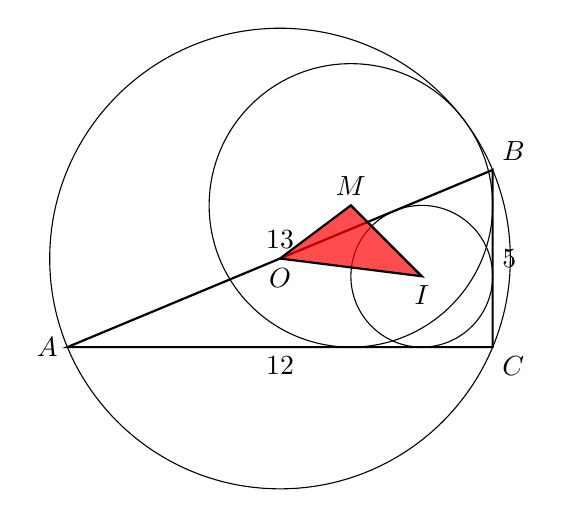
\begin{tikzpicture}[scale=0.45]
    \coordinate (A) at (-12,0);
    \coordinate (B) at (0,5);
    \coordinate (C) at (0,0);
    \coordinate (O) at (-6,2.5);
    \coordinate (I) at (-2,2);
    \coordinate (M) at (-4,4);
    
    \draw[thick] (A)--(B)--(C)--cycle;
    
    \draw (O) circle (6.5);
    
    \draw (I) circle (2);
    
    \draw (M) circle (4);
    
    \fill[red, opacity=0.7] (M)--(O)--(I)--cycle;
    \draw[thick] (M)--(O)--(I)--cycle;
    
    \node[left] at (A) {$A$};
    \node[above right] at (B) {$B$};
    \node[below right] at (C) {$C$};
    \node[below] at (I) {$I$};
    \node[above] at (M) {$M$};
    \node[below] at (O) {$O$};

    \node[above] at ($(A)!0.5!(B)$) {$13$};
    \node[below] at ($(A)!0.5!(C)$) {$12$};
    \node[right] at ($(B)!0.5!(C)$) {$5$};
\end{tikzpicture}
\end{center}
\end{minipage}%
%
\begin{minipage}{0.5\textwidth}
\begin{center}
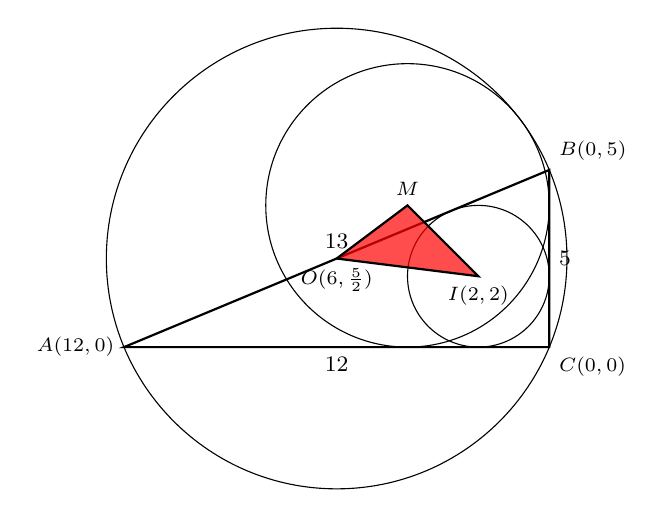
\begin{tikzpicture}[scale=0.45]
    \coordinate (A) at (-12,0);
    \coordinate (B) at (0,5);
    \coordinate (C) at (0,0);
    \coordinate (O) at (-6,2.5);
    \coordinate (I) at (-2,2);
    \coordinate (M) at (-4,4);
    
    \draw[thick] (A)--(B)--(C)--cycle;
    
    \draw (O) circle (6.5);
    
    \draw (I) circle (2);
    
    \draw (M) circle (4);
    
    \fill[red, opacity=0.7] (M)--(O)--(I)--cycle;
    \draw[thick] (M)--(O)--(I)--cycle;
    
    \node[left] at (A) {\scriptsize $A (12, 0)$};
    \node[above right] at (B) {\scriptsize $B (0, 5)$};
    \node[below right] at (C) {\scriptsize $C (0,0)$};
    \node[below] at (I) {\scriptsize $I (2,2)$};
    \node[above] at (M) {\scriptsize $M$};
    \node[below] at (O) {\scriptsize $O (6, \frac{5}{2})$};

    \node[above] at ($(A)!0.5!(B)$) {\footnotesize $13$};
    \node[below] at ($(A)!0.5!(C)$) {\footnotesize $12$};
    \node[right] at ($(B)!0.5!(C)$) {\footnotesize $5$};
\end{tikzpicture}
\end{center}
\end{minipage}

Using the property of incenter, it is evident that the radius of circle $I$ is $2$. Moreover, let the coordinate of $M$ be $(a, a)$. Since $O$ is the circumcenter of $\triangle{ABC}$, the length of $OM$ could be used to find the value of $a$.
\begin{align*}
    \sqrt{(a - 6)^2 + \left( a - \frac{5}{2} \right)^2} &= \frac{13}{2} - a \\
    2a^2 - 17a + 36 + \frac{25}{4} &= a^2 - 13a + \frac{169}{4} \\
    a^2 - 4a &= 0 \\
    \therefore a &= 4
\end{align*}
The area of $\triangle{IMO}$ could be computed using the Shoelace formula.
\begin{align*}
    [IMO]
    &= \frac{1}{2}
    \begin{vmatrix}
        2 & 4 & 6 & 2 \\
        2 & 4 & \frac{5}{2} & 2
    \end{vmatrix} \\
    &= \frac{1}{2} \left| (8 + 10 + 12) - (8 + 24 + 5) \right| \\
    &= \boxed{\textbf{(E)}\ \frac72}
\end{align*}
\end{solution}

\end{document}
